\section{Die Sturmwarnung}\Diskussionspunkt{zu webseite hinzu oder einzelnes Kapitel zusammen mit notification?}

Die Seite mir der Sturmwarnung, siehe \ref{img:Sturmwarnung} auf Seite \pageref{img:Sturmwarnung} gibt es im eigentlichen nicht mehr, dies wurde beginn November umgestellt aus Sicherheitsgründen, welche in der Problemanalyse erläutert werden. Zum jetzigen Zeitpunkt wird nur noch ein Link zur Verfügung gestellt um auf die kantonale Sturmwarnseite zu kommen. Die Daten dieser Seite werden mit dem deutschen Wetterdienst in Stuttgart sowie Meteo Schweiz erstellt und dienen auf der Webseite nur als Information. Es sollte vor Ort beachtet werden ob die Warnlampen eingeschalten sind. Zu beachten ist hierbei, dass die Sturmwarnungen Bürozeiten haben. D.h. konkret vom 1. April bis 31 Oktober zwischen 6 und 22 Uhr und vom 1. November bis 31. März zwischen 7 und 20 Uhr. Der deutsche Wetterdienst und Meteo Schweiz unterscheiden zwei verschiedene Kategorien. Zum einen starke Windböen zwischen 25 und 33 Knoten, dies wird 40 Blitze pro Minute an den Leuchten signalisiert. Zum anderen Sturmböen von 34 und mehr Knoten, welche mit 90 Blitze pro Minute signalisiert werden. Zusätzlich zu den beiden Kategorien wird der Bodensee in 3 verschiedene Zonen unterteilt, West, Mitte und Ost, wobei Arbon in zur Zone Ost gehört. 
\begin{figure}[htbp]
	\centering
	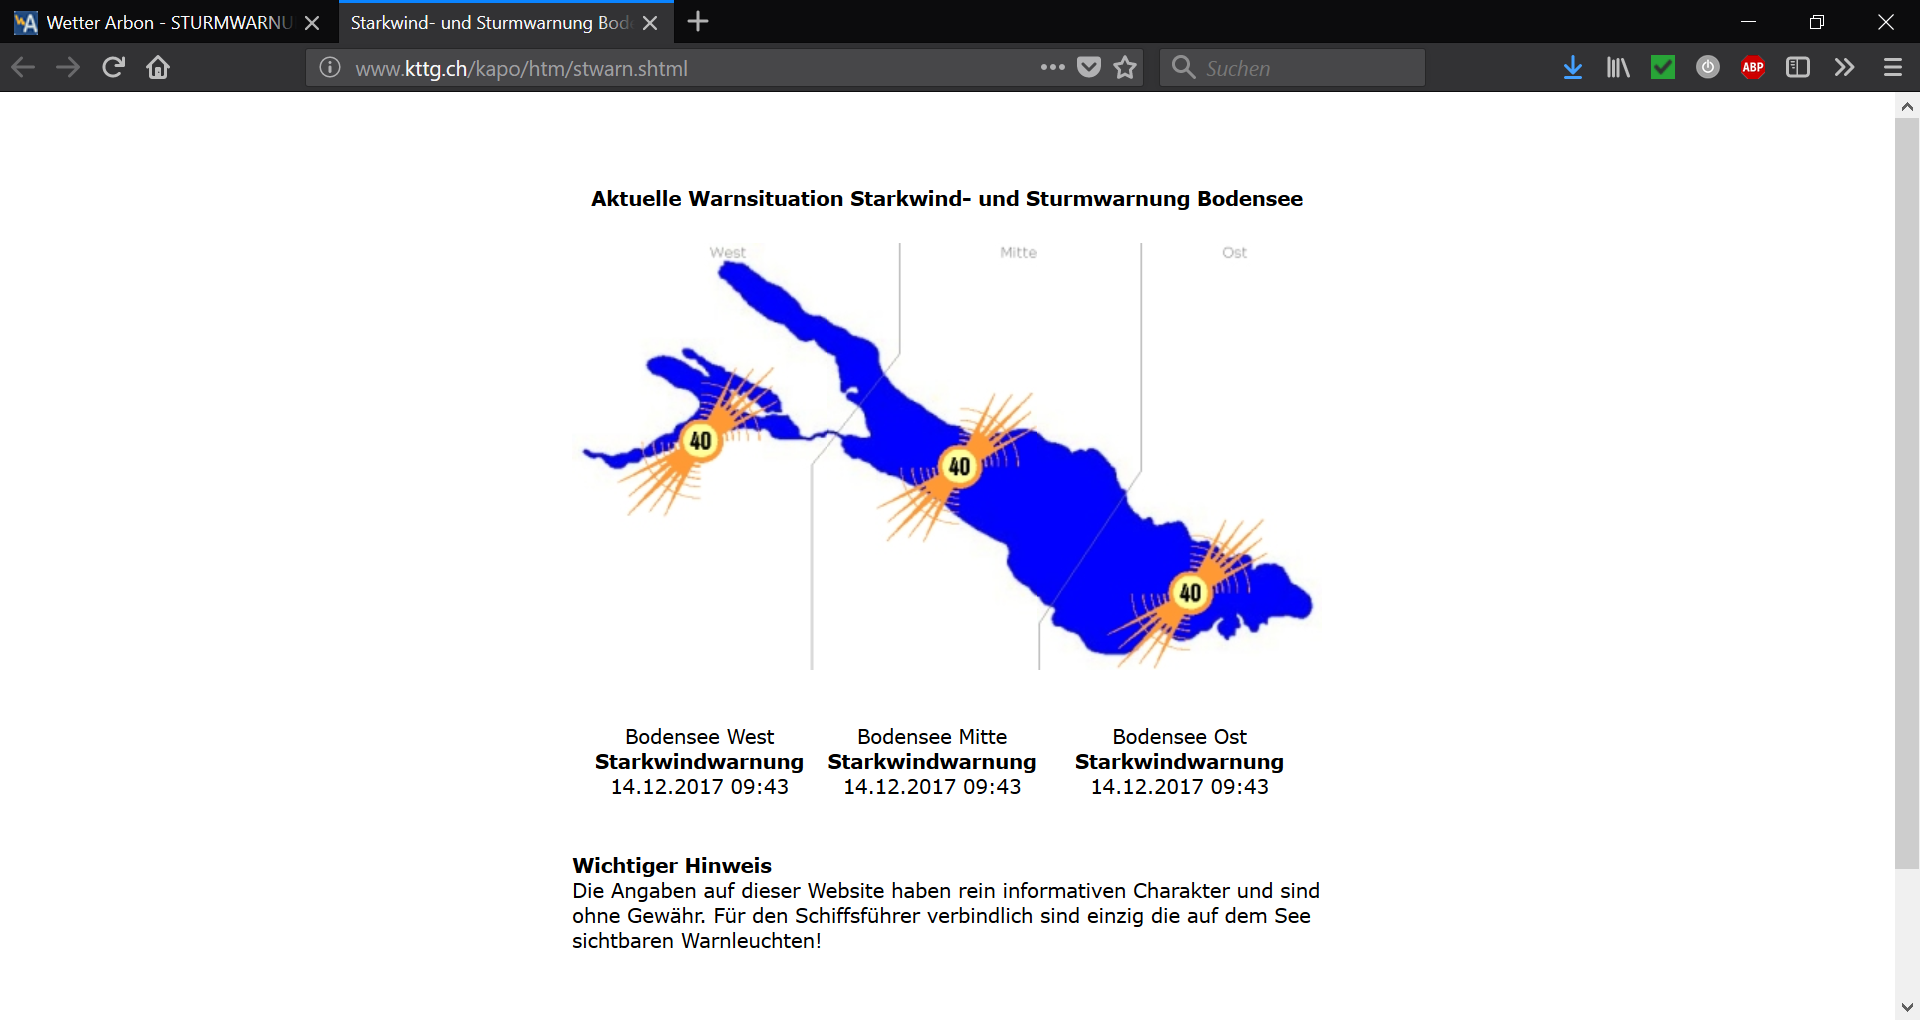
\includegraphics[width=0.9\linewidth]{img/sturmwarnung}
	\caption{Sturmwarnung vom Kanton Thurgau}
	\label{img:Sturmwarnung}
\end{figure}

Wie schon erklärt ist das Problem hierbei der HTTP Standard, viele der Webbrowser stellen die Unterstützung dieses Standards langsam aber sicher ein und werden dann nur noch HTTPS unterstützen\cite{Mozilla:DeprecatingNon-SecureHTTP}. Deswegen ist die Sturmwarnung nur über einen Link aufrufbar. Des Weiteren wurde öfters der Wunsch nach einer SMS-Benachrichtigung geäussert, dies ist momentan nicht realisiert und soll auch teil unserer BA sein. 

Die Sturmwarnung soll wieder auf der Webseite sichtbar sein und der Besucher der Webseite soll die Möglichkeit haben sich für eine Notification zu registrieren. Dafür wurden 3 verschiedene Möglichkeiten ausgewählt und mit der Nutzwertanalyse ausgewertet. Ziel bei allen Möglichkeiten ist es, dass der Benutzer die Möglichkeit hat sich zu registrieren und Alarmkriterien zu bestimmen. Werden die gewählten Alarmkriterien erreicht bzw. wird eine Sturmwarnung herausgegeben, wird der Benutzer benachrichtigt. Hiermit soll die Möglichkeit gegeben werden, dass der Benutzer in Echtzeit informiert wird und somit keine Warnung oder sein "perfektes" Segelwetter verpasst. Für die evaluierung der Notifications wurde eine Nutzwertanalyse erstellt. Dies ist eine gute Möglichkeit, um verschiedene Lösungsansätze zu bewerten. Der Nachteil hierbei ist jedoch, dass die Bewertung sehr subjektiv ist. 

\begin{center}
\begin{tabular}{ |p{3.5cm}||p{1cm}|p{2cm}|p{3.5cm}|p{2.5cm}|p{1.5cm}|}
 \hline
 \multicolumn{6}{|c|}{Nutzwertanalyse} \\
 \hline
	Möglichkeiten & Kosten & Einfachheit & Programmieraufwand & Anpassbarkeit & Support\\
 \hline
	SMS & 1 & 4 & 3 & 3 & 5\\
	E-Mail & 5 & 4 & 5 & 5 & 1\\
	FacebookMessenger & 5 & 4 & 3 & 4 & 1\\
 
\hline
\end{tabular}
\end{center}

Aus der Nutzwertanalyse ist Sichtbar, dass die Benachrichtigung per E-Mail und Facebook Messenger die Lösungsansätze mit der höchsten Punktzahl sind . Der grösste Vorteil der beiden möglichen Lösungen sind, dass sie Kostenlos sind. Der Nachteil an Facebook Messenger ist, das nicht davon ausgegangen werden kann, dass jeder Benutzer ein Facebookprofil hat. 
